\documentclass[]{book}
\usepackage{lmodern}
\usepackage{amssymb,amsmath}
\usepackage{ifxetex,ifluatex}
\usepackage{fixltx2e} % provides \textsubscript
\ifnum 0\ifxetex 1\fi\ifluatex 1\fi=0 % if pdftex
  \usepackage[T1]{fontenc}
  \usepackage[utf8]{inputenc}
\else % if luatex or xelatex
  \ifxetex
    \usepackage{mathspec}
  \else
    \usepackage{fontspec}
  \fi
  \defaultfontfeatures{Ligatures=TeX,Scale=MatchLowercase}
\fi
% use upquote if available, for straight quotes in verbatim environments
\IfFileExists{upquote.sty}{\usepackage{upquote}}{}
% use microtype if available
\IfFileExists{microtype.sty}{%
\usepackage{microtype}
\UseMicrotypeSet[protrusion]{basicmath} % disable protrusion for tt fonts
}{}
\usepackage[margin=1in]{geometry}
\usepackage{hyperref}
\hypersetup{unicode=true,
            pdftitle={MTXQCvX2 documentation},
            pdfauthor={Christin Zasada},
            pdfborder={0 0 0},
            breaklinks=true}
\urlstyle{same}  % don't use monospace font for urls
\usepackage{natbib}
\bibliographystyle{apalike}
\usepackage{color}
\usepackage{fancyvrb}
\newcommand{\VerbBar}{|}
\newcommand{\VERB}{\Verb[commandchars=\\\{\}]}
\DefineVerbatimEnvironment{Highlighting}{Verbatim}{commandchars=\\\{\}}
% Add ',fontsize=\small' for more characters per line
\usepackage{framed}
\definecolor{shadecolor}{RGB}{248,248,248}
\newenvironment{Shaded}{\begin{snugshade}}{\end{snugshade}}
\newcommand{\KeywordTok}[1]{\textcolor[rgb]{0.13,0.29,0.53}{\textbf{#1}}}
\newcommand{\DataTypeTok}[1]{\textcolor[rgb]{0.13,0.29,0.53}{#1}}
\newcommand{\DecValTok}[1]{\textcolor[rgb]{0.00,0.00,0.81}{#1}}
\newcommand{\BaseNTok}[1]{\textcolor[rgb]{0.00,0.00,0.81}{#1}}
\newcommand{\FloatTok}[1]{\textcolor[rgb]{0.00,0.00,0.81}{#1}}
\newcommand{\ConstantTok}[1]{\textcolor[rgb]{0.00,0.00,0.00}{#1}}
\newcommand{\CharTok}[1]{\textcolor[rgb]{0.31,0.60,0.02}{#1}}
\newcommand{\SpecialCharTok}[1]{\textcolor[rgb]{0.00,0.00,0.00}{#1}}
\newcommand{\StringTok}[1]{\textcolor[rgb]{0.31,0.60,0.02}{#1}}
\newcommand{\VerbatimStringTok}[1]{\textcolor[rgb]{0.31,0.60,0.02}{#1}}
\newcommand{\SpecialStringTok}[1]{\textcolor[rgb]{0.31,0.60,0.02}{#1}}
\newcommand{\ImportTok}[1]{#1}
\newcommand{\CommentTok}[1]{\textcolor[rgb]{0.56,0.35,0.01}{\textit{#1}}}
\newcommand{\DocumentationTok}[1]{\textcolor[rgb]{0.56,0.35,0.01}{\textbf{\textit{#1}}}}
\newcommand{\AnnotationTok}[1]{\textcolor[rgb]{0.56,0.35,0.01}{\textbf{\textit{#1}}}}
\newcommand{\CommentVarTok}[1]{\textcolor[rgb]{0.56,0.35,0.01}{\textbf{\textit{#1}}}}
\newcommand{\OtherTok}[1]{\textcolor[rgb]{0.56,0.35,0.01}{#1}}
\newcommand{\FunctionTok}[1]{\textcolor[rgb]{0.00,0.00,0.00}{#1}}
\newcommand{\VariableTok}[1]{\textcolor[rgb]{0.00,0.00,0.00}{#1}}
\newcommand{\ControlFlowTok}[1]{\textcolor[rgb]{0.13,0.29,0.53}{\textbf{#1}}}
\newcommand{\OperatorTok}[1]{\textcolor[rgb]{0.81,0.36,0.00}{\textbf{#1}}}
\newcommand{\BuiltInTok}[1]{#1}
\newcommand{\ExtensionTok}[1]{#1}
\newcommand{\PreprocessorTok}[1]{\textcolor[rgb]{0.56,0.35,0.01}{\textit{#1}}}
\newcommand{\AttributeTok}[1]{\textcolor[rgb]{0.77,0.63,0.00}{#1}}
\newcommand{\RegionMarkerTok}[1]{#1}
\newcommand{\InformationTok}[1]{\textcolor[rgb]{0.56,0.35,0.01}{\textbf{\textit{#1}}}}
\newcommand{\WarningTok}[1]{\textcolor[rgb]{0.56,0.35,0.01}{\textbf{\textit{#1}}}}
\newcommand{\AlertTok}[1]{\textcolor[rgb]{0.94,0.16,0.16}{#1}}
\newcommand{\ErrorTok}[1]{\textcolor[rgb]{0.64,0.00,0.00}{\textbf{#1}}}
\newcommand{\NormalTok}[1]{#1}
\usepackage{longtable,booktabs}
\usepackage{graphicx,grffile}
\makeatletter
\def\maxwidth{\ifdim\Gin@nat@width>\linewidth\linewidth\else\Gin@nat@width\fi}
\def\maxheight{\ifdim\Gin@nat@height>\textheight\textheight\else\Gin@nat@height\fi}
\makeatother
% Scale images if necessary, so that they will not overflow the page
% margins by default, and it is still possible to overwrite the defaults
% using explicit options in \includegraphics[width, height, ...]{}
\setkeys{Gin}{width=\maxwidth,height=\maxheight,keepaspectratio}
\IfFileExists{parskip.sty}{%
\usepackage{parskip}
}{% else
\setlength{\parindent}{0pt}
\setlength{\parskip}{6pt plus 2pt minus 1pt}
}
\setlength{\emergencystretch}{3em}  % prevent overfull lines
\providecommand{\tightlist}{%
  \setlength{\itemsep}{0pt}\setlength{\parskip}{0pt}}
\setcounter{secnumdepth}{5}
% Redefines (sub)paragraphs to behave more like sections
\ifx\paragraph\undefined\else
\let\oldparagraph\paragraph
\renewcommand{\paragraph}[1]{\oldparagraph{#1}\mbox{}}
\fi
\ifx\subparagraph\undefined\else
\let\oldsubparagraph\subparagraph
\renewcommand{\subparagraph}[1]{\oldsubparagraph{#1}\mbox{}}
\fi

%%% Use protect on footnotes to avoid problems with footnotes in titles
\let\rmarkdownfootnote\footnote%
\def\footnote{\protect\rmarkdownfootnote}

%%% Change title format to be more compact
\usepackage{titling}

% Create subtitle command for use in maketitle
\newcommand{\subtitle}[1]{
  \posttitle{
    \begin{center}\large#1\end{center}
    }
}

\setlength{\droptitle}{-2em}

  \title{MTXQCvX2 documentation}
    \pretitle{\vspace{\droptitle}\centering\huge}
  \posttitle{\par}
    \author{Christin Zasada}
    \preauthor{\centering\large\emph}
  \postauthor{\par}
      \predate{\centering\large\emph}
  \postdate{\par}
    \date{2018-11-01}

\usepackage{booktabs}

\usepackage{amsthm}
\newtheorem{theorem}{Theorem}[chapter]
\newtheorem{lemma}{Lemma}[chapter]
\theoremstyle{definition}
\newtheorem{definition}{Definition}[chapter]
\newtheorem{corollary}{Corollary}[chapter]
\newtheorem{proposition}{Proposition}[chapter]
\theoremstyle{definition}
\newtheorem{example}{Example}[chapter]
\theoremstyle{definition}
\newtheorem{exercise}{Exercise}[chapter]
\theoremstyle{remark}
\newtheorem*{remark}{Remark}
\newtheorem*{solution}{Solution}
\begin{document}
\maketitle

{
\setcounter{tocdepth}{1}
\tableofcontents
}
\chapter{Welcome}\label{welcome}

This documentation introduced to you how to use MTXQCvX2 in order to
assess the quality of your GC-MS derived data, perform the determination
of calibration curves and absolute quantification. It furthermore
provides you two normalisation strategies and the calculation of
quantities in, e.g., pmol/1e+6 cells or pmol/mg tissue.

MTXQCvX2 does also enable the calculation of stable isotopic
incorporation and the evaluation of the underlying data, the mass
isotopomer distributions (MIDs).

The tool has been set up to support the in-lab developed workflow for
quantitative metabolomics experiments using the in-house developed
software Maui for the annotation of data. MTXQCvX2 bridges the gap
between quality control and first data post-processing / analysis of
GC-MS derived data (MTXQCvX2\_part1, MTXQCvX2\_part2).

Nevertheless MTXQCvX2 includes a module in order to integrate all kind
of data provided in spreadsheet-format, e.g., derived from metmax,
extracting required information and creating corresponding files
(MTXQCvX2\_part4).

Both workflows are introduced in the distinct chapters including their
required input parameter (chapter \protect\hyperlink{wf:maui}{Workflow
Maui} and \protect\hyperlink{wf:metmax}{Workflow Metmax}).

\chapter{Introduction}\label{intro}

Experimental and mathematical concepts have been introduced for the
pulsed stable isotope resolved metabolomics (pSIRM) approach in
\citep{Pietzke2014}.

\begin{Shaded}
\begin{Highlighting}[]
\NormalTok{knitr}\OperatorTok{::}\KeywordTok{include_graphics}\NormalTok{(}\StringTok{"images/now.png"}\NormalTok{)}
\end{Highlighting}
\end{Shaded}

\begin{figure}
\centering
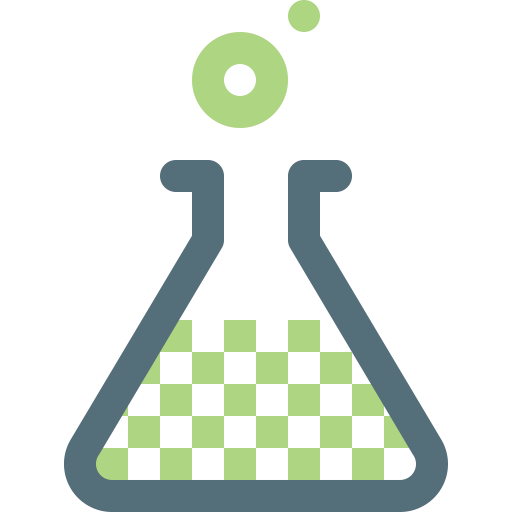
\includegraphics{images/now.png}
\caption{\label{fig:flow}Test external figure and how to include it}
\end{figure}

\hypertarget{wf:maui}{\chapter{Workflow for Maui-annotation
projects}\label{wf:maui}}

\section{Read this in case}\label{read-this-in-case}

\begin{itemize}
\tightlist
\item
  you have run a Maui project
\item
  exported all required container (see \ref{container})
\item
  you have a copy of sequence list and experimental conditions
\item
  you know the extraction procedure
\end{itemize}

The following article describes briefly how to use MTXQCvX2 in case you
used Maui for the annotation of your metabolomics project. It does not
matter if you have performed an experiment including stable isotopes or
if you just aim for the quantification of a few intermediates.

\section{Quick view}\label{quick-view}

\begin{enumerate}
\def\labelenumi{\arabic{enumi}.}
\tightlist
\item
  Setup a new R-project and copy MTXQC template files and folders
\item
  Knit with parameter: \texttt{MTXQC\_init.Rmd} and create project
  folder, e.g., \texttt{psirm\_glucose}
\item
  Copy input files and rename \texttt{ManualQuantTable.tsv}
  (e18205cz.tsv)
\item
  Create \texttt{annotation.csv} and \texttt{sample\_extracts.csv} files
\item
  Define the internal extraction standard
\item
  Knit with parameter: \texttt{MTXQC\_ExperimentalSetup.Rmd}
\item
  Knit with parameter: \texttt{MTXQC\_part1.Rmd}
\item
  Knit with parameter: \texttt{MTXQC\_part2.Rmd}
\item
  If required, proceed with \texttt{MTXQC\_part3.Rmd} for
  ManualValidation
\end{enumerate}

\section{Input files}\label{input-files}

Three different kind of export functions have been implemented in Maui.
These functions provide the export of the actual data into \texttt{.csv}
or \texttt{.tsv} files that are directly usable as input files for
MTXQCvX2. Please refer to section \ref{mauiexport} how you perform the
export and which containers have to be exported using what export
function and where to copy them in \texttt{psirm\_glucose/input/}.

Certain circumstances might wish you to combine \emph{multiple
MAUI-projects} into one MTXQC-project. This might be the case when you
run the same samples in split and splitless mode on the machine or your
experimental setup has been measured in multiple batches in order to
avoid derivatisation effects.

It is highly recommended to combine the input files derived from a
different Maui projects beforehand the analysis. In that way you have
only to work with a single file
\texttt{CalculationFileData.csv}\footnote{stored in
  \texttt{psirm\_glucose/output/quant/...}} containing all data of the
your experiment.

The herein described process provides a quick way how to combine the
exported files from different Maui projects. The script
\texttt{combine-sets.R}\footnote{inst/template\_files/\ldots{}}
automatically saves all combined files into the correct \texttt{input}
folder. Just update the folder and subfolder names. All the rest has
been taken care of for you.

\begin{enumerate}
\def\labelenumi{\arabic{enumi}.}
\tightlist
\item
  Create in the MTXQC-project folder (e.g., \texttt{psirm\_glucose/}) a
  new folder called \texttt{raw-data}
\item
  Create a subfolder for each Maui-project in
  \texttt{psirm\_glucose/raw\_data/...}
\item
  Copy into this folder all your Maui-derived input files altogether
\item
  Update the parameter of \texttt{combine-sets.R}, meaning folder name
  definitions, file
\item
  Execute the R script
\item
  Merged files have been generated and copied into the corresponding
  folder: \texttt{psirm\_glucose/input-folder/gc/...} or
  \texttt{psirm\_glucose/input-folder/inc/...}
\item
  Copy the renamed \texttt{ManualQuantTable.tsv} files of each Maui
  project into \texttt{psirm\_glucose/input/quant/...}
\end{enumerate}

\section{Annotation-file}\label{annotation-file}

The annotation file relate file names with experimental conditions or
specify quantification standards in your batch. Two columns -
\textbf{File and Type} - are obligatory and have to be present in the
annotation file. In the case of their absence
\texttt{MTXQCvX\_part1.Rmd} stops processing and shows an error message.

A quick way to generate an annotation file is described below:

\begin{enumerate}
\def\labelenumi{\arabic{enumi}.}
\tightlist
\item
  Copy the first row / header of \texttt{quantMassAreaMatrix.csv} file
\item
  Paste \& transpose the content into a new Excel-File into column A
\item
  Change the first entry: Metabolite -\textgreater{} File
\item
  Remove the entry QuantMasses at the very end of the column A
\item
  Add the column Type and specify each file either as \textbf{sample} or
  \textbf{addQ1\_dilution}\footnote{see for further details
    additionalQuant}
\item
  Add more columns specifying your experimental conditions, e.g.,
  Cellline and Treatment\footnote{optimal: two-three parameter, max:
    four parameter. Consider possible combinations, e.g.,
    HCT116-control, HCT116-BPTES}
\item
  Save the content as \texttt{csv-file} in the
  \texttt{psirm\_glucose/input/...}
\end{enumerate}

\section{Sample\_extracts-file}\label{sample_extracts-file}

The \texttt{sample\_extracts.csv} file is required in order to determine
automatically absolute quantities in the manner of pmol/1e+6 cells or
pmol/mg tissue in the \texttt{CalculationFileData.csv}.

This file requires two obligatory columns - \textbf{Extract\_vol} and
\textbf{Unit}\footnote{Define: count, mg or ul}. Please specify for each
experimental condition the amount of extracted cells (count), tissue
(mg) or volume of blood/plasme (ul) in the unit shown in the brackets.\\
The names of the columns of the experimental conditions have to match up
with the annotation file. Save the file in the folder
\texttt{psirm\_glucose/input/...}.

If the defined experimental conditions do not match up with the
annotation \texttt{MTXQCvX2\_part1.Rmd} exit data processing. A template
file is saved for review and usage at \texttt{inst/template\_files/...}

\section{Internal Standard}\label{internal-standard}

MTXQCvX2 allows the specification of project-specific internal
extraction standards. The only thing you need to do is to define the
corresponding compounds as an internal standard in the
\texttt{conversion\_metabolite.csv} file. To do so, add
\texttt{InternalStandard} to the compound in last column
\texttt{Standard}.

For an classical pSIRM experiment in the Kempa lab we are using cinnamic
acid. The evaluation of this compound has been integrated in Maui. Peak
areas of cinnamic acid are exported from a distinct container called
\texttt{cinAcid}. The exported file has to be renamed to
\texttt{InternalStandard.csv} though and moved to
\texttt{psirm\_glucose/input/gc/...}.

If you have used a different compound as an internal extraction standard
you might need to extract the peak areas of this compound from the Maui
export file \texttt{quantPeakAreasMatrix.csv} file and save it in the
folder \texttt{psirm\_glucose/input/gc/InternalStandard.csv},
respectively. Prerequisite - you have annotated the compound in Maui.

The report of \texttt{MTXQCvX2\_part1.Rmd} includes the defined internal
standard for each project in a message.

\hypertarget{wf:metmax}{\chapter{Workflow for Metmax-extracted
projects}\label{wf:metmax}}

\section{You want to follow this
\ldots{}}\label{you-want-to-follow-this}

\begin{itemize}
\tightlist
\item
  in case you have measured samples and quantification standards by
  GC-MS
\item
  performed the annotation of intermediates in ChromaToF or vendor
  software
\item
  exported all information into \texttt{.txt} files
\item
  used metmax to extract peak areas / mass isotopomer distributions
  (MIDs)
\end{itemize}

\section{Introduction}\label{introduction}

This document describes how to use MTXQCvX2 in combination with
metmax\footnote{\url{http://gmd.mpimp-golm.mpg.de/apps/metmax/default.htm}}.

Historically, MTXQCvX2 has been developed and optimized for Maui-derived
input files. The \texttt{MTXQCvX2-part4.Rmd} functions as a converter of
metmax-derived files in order to create suitable input formats for
\texttt{MTXQCvX-part1.Rmd}.

This module could also be used to convert tables derived from other
programs as long as they are stick with the herein described table
formats. Mandatory columns are referenced in the text for each kind of
input file.

The general workflow of the NMTXQCvX2 project is briefly shown below in
quick view. More detailed instructions are summarised in the following
paragraphs.

For more detailed explanations about the individual input parameter for
each module of MTXQCvX2 please proceed to read the documentation about
the individual modules and their knitting parameter. The relation of
knitting parameter, input and output files are described in each
section.

\section{Quick view}\label{quick-view-1}

\begin{enumerate}
\def\labelenumi{\arabic{enumi}.}
\tightlist
\item
  Generate input files: run \texttt{MTXQC\_part4.Rmd}\footnote{read here
    the instructions}
\item
  Setup R-project and copy MTXQC-files
\item
  Knit with parameter: \texttt{MTXQC\_init.Rmd}
\item
  Copy input files into corresponding folders
\item
  Create annotation.csv and sample\_extracts.csv files\footnote{Details
    further down this document}
\item
  Update metabolite names in
  \texttt{conversion\_metabolite.csv}\footnote{Column:
    Metabolite\_manual}
\item
  Define the internal standard and/or alkanes\footnote{Also in
    conversion\_metabolite.csv; see below paragraph Standards}
\item
  Knit with parameter: \texttt{MTXQC\_ExperimentalSetup.Rmd}
\item
  Knit with parameter: \texttt{MTXQC\_part1.Rmd}
\item
  Knit with parameter: \texttt{MTXQC\_part2.Rmd}
\item
  If required - proceed with \texttt{MTXQC\_part3.Rmd} for
  ManualValidation
\end{enumerate}

\section{Input files}\label{input-files-1}

If you need an introduction about how to use metmax - have a look at the
separate documentation \texttt{Metmax\_intro}.

The chapter \ref{part4} \texttt{MTXQCvX\_part4} explains in detail how
to use this module to generate suitable input files.

\section{Annotation-file}\label{annotation-file-1}

The annotation file relate file names with experimental conditions or
specify quantification standards in your batch. Two columns -
\textbf{File and Type} - are obligatory and have to be present in the
annotation file. In the case of their absence
\texttt{MTXQCvX\_part1.Rmd} stops processing and shows an error message.

A quick way to generate an annotation file is described below:

\begin{enumerate}
\def\labelenumi{\arabic{enumi}.}
\tightlist
\item
  Copy all file names from a file of your choice
\item
  Paste \& transpose the content into a new Excel-File into column A
\item
  Call column A -\textgreater{} File
\item
  Optional: Remove any non-file name entry in this column
\item
  Add the column Type and specify each file either as \textbf{sample},
  \textbf{Q1\_diluation}, ,\textbf{addQ1\_dilution}\footnote{see for
    further details additionalQuant}
\item
  Add more columns specifying your experimental conditions, e.g.,
  Cellline and Treatment\footnote{optimal: two-three parameter, max:
    four parameter. Consider possible combinations, e.g.,
    HCT116-control, HCT116-BPTES}
\item
  Save the content as \texttt{csv-file} in the
  \texttt{psirm\_glucose/input/...}
\end{enumerate}

\section{Sample\_extracts-file}\label{sample_extracts-file-1}

The \texttt{sample\_extracts.csv} file is required in order to determine
automatically absolute quantities in the manner of pmol/1e+6 cells or
pmol/mg tissue in the \texttt{CalculationFileData.csv}.

This file requires two obligatory columns - \textbf{Extract\_vol} and
\textbf{Unit}\footnote{Define: count, mg or ul}. Please specify for each
experimental condition the amount of extracted cells (count), tissue
(mg) or volume of blood/plasme (ul) in the unit shown in the brackets.\\
The names of the columns of the experimental conditions have to match up
with the annotation file. Save the file in the folder
\texttt{psirm\_glucose/input/...}.

If the defined experimental conditions do not match up with the
annotation \texttt{MTXQCvX2\_part1.Rmd} exit data processing. A template
file is saved for review and usage at \texttt{inst/template\_files/...}

\section{\texorpdfstring{Update metabolite names in
\texttt{conversion\_metabolite.csv}}{Update metabolite names in conversion\_metabolite.csv}}\label{update-metabolite-names-in-conversion_metabolite.csv}

The file \texttt{conversion\_metabolite.csv}, saved in
\texttt{config\_mtx/}, serves as a kind of translational table. It
defines alternative version of metabolite library names that come in
handy to plot data using shorter metabolite names. This file is also
used to define settings and standard classifications. Detailed
information for each column of the file are shown here: REF

\subsection{Match your annotation with library
names}\label{match-your-annotation-with-library-names}

Prior the analysis you need to match the names of your intermediates
with the conversion\_metabolite.csv file. You need to update or add the
corresponding name for each intermediate in the column
\textbf{Metabolite\_manual}.

General suggestion for naming conventions in ChromaToF:
Metabolite\_Derivate, e.g., Lactic acid\_(2TMS). In case of the presence
of main- (MP) and byproducts (BP) use: Metabolite\_Derivate\_MP/BP,
e.g., Glucose\_(1MEOX)(5TMS)\_MP.

If you have annotated intermediates that are not included so far in this
table please follow the instructions how to extend
\texttt{conversion\_metabolite.csv}.REF

\subsection{Define your internal standards and
alkanes}\label{define-your-internal-standards-and-alkanes}

MTXQCvX2 allows the specification of project-specific internal
standards. Corresponding compounds have to be marked as an internal
standard in \texttt{conversion\_metabolite.csv} by adding the tag
\textbf{InternalStandard} in the column Standard.

If you check the box - InternalStandard in the parameter selection for
\texttt{MTXQCvX2\_part4.Rmd} the module searches in your input file for
peak areas of the defined standard and extracts the information. It also
generates the file \texttt{InternalStandard.csv} and stores it at
\texttt{psirm\_glucose/input/gc/...}.

In the same way alkanes are defined in
\texttt{conversion\_metabolite.csv}. Each alkane has to be flag tagged
with \textbf{Alk} in the column Standard. This gives you the opportunity
to implement customized mixtures of alkanes in order to determine the
retention index. \texttt{MTXQCvX\_part4.Rmd} recognises the flag tag and
generates \texttt{Alcane\_intensities.csv} based on your input file
containing peak areas and saves it in
\texttt{psirm\_glucose/input/gc/...}\footnote{It should be
  al\textbf{k}ane, I know, but Maui doesn't, unfortunately\ldots{}}.

The in-lab protocol considers nine alkanes from c10 to c36. Standard
annotation includes an hashtag, e.g., \#c10. If you use this annotation
even Metmax would be able to determine the retention index.

\chapter{MTXQCvX2 Universe}\label{universe}

Back then in 2015 I started to think about a way how to evaluate my own
datasets regarding some quality parameters. From a scratch of a few
quality metrices evaluated in the frame of a very, very long Rscript
until now many different generations of the MTXQC existed.

Out of this evolution cycle MTXQC developed to a suit of modules that
can be used complimentary in order to evaluate and process GC-MS derived
metabolomics data. \texttt{MTXQC\_part1.Rmd} represents the heart of
this little universe. Besides that there are many ways how to use
MTXQCvX2. Proposed workflows are illustrated in chapter
\protect\hyperlink{wf:maui}{Workflow Maui} and chapter
\protect\hyperlink{wf:metmax}{Workflow Metmax}. The flow diagram
introduced \href{/ref@fig:flow}{here} might help you to decide how to
get started.

The following sections give a short overview about the main parameters
and functions of each module, its generated graphical illustrations and
tables.

\section{MTXQC\_init.Rmd}\label{init}

\section{MTXQC\_ExperimentalSetup}\label{expsetup}

\section{MTXQC\_part 1}\label{heart}

\section{MTXQC\_part 2 - Post-Processing}\label{postproc}

\section{MTXQC\_part 3 - Manual Validation}\label{manval}

\section{MTXQC\_part 4 - Metmax integration}\label{metmax}

\chapter{\texorpdfstring{Configuration of MTXQCvX2 -
\texttt{config\_mtx/...}}{Configuration of MTXQCvX2 - config\_mtx/...}}\label{configuration-of-mtxqcvx2---config_mtx...}

Herein explained are the customizable tables of the MTXQCvX2 universe.

\section{\texorpdfstring{\texttt{conversion\_metabolite.csv}}{conversion\_metabolite.csv}}\label{conversion_metabolite.csv}

Column.name

Description

Value

Metabolite\_manual

Manual defined metabolite name

\#Alanine (2TMS)

Metabolite

Library name of the metabolite

Alanine\_(2TMS)\_BP\_RI:1097\_IDENT:B+C

Metabolite\_short

Short version of library name of the metabolite

Alanine\_(2TMS)

Lettercode

Lettercode version of metabolite name

Ala\_2TMS

Q1\_value

Checked if quant1:1 value available

x

Mass\_Pos

m/z-value corresponding to m\_inc

118

SE\_sel

Evaluation of the MIDs

x

Q\_sel

Evaluation for absolute quantification

x

nopsirm

Exclusively for absolute quantification

Standards

Defined as standard

InternalStandard, Alk

\section{\texorpdfstring{\texttt{letter\_pathway\_complete.csv}}{letter\_pathway\_complete.csv}}\label{letter_pathway_complete.csv}

Column.name

Description

Value

Letter\_Derivate

Derivate definition

Ala

Lettercode

Lettercode name of metabolite

Ala\_3TMS

Pathway

Ass.pathway

aa

Pathway.1

Ass. pathway - ordered for heatmap

5-aa

Met\_pathway

Ass. pathway - ordered for heatmap incl. Lettercode

5-aa\_Ala\_3TMS

Subs\_class

Substance class

aa

Met\_class

Substance class incl. Lettercode

aa\_Ala\_3TMS

\section{\texorpdfstring{\texttt{quant1-values.csv}}{quant1-values.csv}}\label{quant1-values.csv}

Column.name

Description

Value

Letter\_Derivate

Derivate name of metabolite

3PGA

Quant1\_v4

Quantity in (pmol)

43480

Quant1\_v3

Quantity in (pmol)

43480

\section{\texorpdfstring{\texttt{incorporation\_calc.csv} \&
\texttt{mid\_backups.csv}}{incorporation\_calc.csv \& mid\_backups.csv}}\label{incorporation_calc.csv-mid_backups.csv}

Column.name

Description

Value

Metabolite

Library name of metabolite

Alanine\_(2TMS)\_BP\_RI:1097\_IDENT:B+C

Mass\_mz

m/z-value

116, 118

LI\_MID

Definition of mass level

m0, minc

Column.name

Description

Value

Metabolite

Library name of metabolite

Alanine\_ beta-\_(3TMS)\_MP\_RI:1435\_IDENT:A+D

Mass.m.z.

m/z value

188

BackupPeakArea

Peak area of Backup MID

4960

BackupMID

MID value for corresponding Mass.m.z.

0.8005

\chapter{pSIRM experiments}\label{psirm}

The application of stable isotopes provides a powerful tool to track the
activity of metabolic pathways. the time-dependent and atom-specific
routing along a metabolic pathway resolved how substrates like glucose
or glutamine are used in order to maintain a certain phenotype and
energetic homeostatsis.

We developed an approach called pulsed stable isotope resolved
metabolomics (pSIRM) enabling the quantitative evaluation of metabolite
pool sizes and incorporation of stable isotopes, e.g.,
\(^{13}C_6\)-glucose. A thoughtful setup of the experimental design
including the applied substrates and carefull experimental handling are
prerequisites for a successful pSIRM experiment. Essential aspects are
collected in the below paragraphs along with a number of usefull tweaks.

\section{Experimental design}\label{experimental-design}

An \emph{in vitro} pSIRM experiment lasts in total up to three days
starting from the cell seeding at day zero. Further along the way up to
two media changes should be included until the application of stable
isotopes and harvesting the cells maintaining the continouse
availability of nutrients and avoiding the accumulation of waste
products (Figure \ref(fig:psirm)). The media change four hours prior the
harvest is set up in order to give cells time to recover from the
mechanical stress of the media change. At the time point of harvest
cells should be in a perfect happily state regarding metabolic
environment and stress.

Choose carefully the \emph{seeding density of you cells} in the first
place. High confluency inducing contact inhibition of cell growth has a
strong impact on several cellular processes including the uptake of
nutrients. Try to aim for petri dishes with a maximum confluency of
75-80 \%. A pre-experiment including different cell densities for
seeding at a number of experimental conditions helps you to get a
feeling for the cell growth in general and an expected output of cells
at the time point of the harvest. Later one is useful to plan sample
extraction and measurement subsequently.

\begin{figure}
\centering
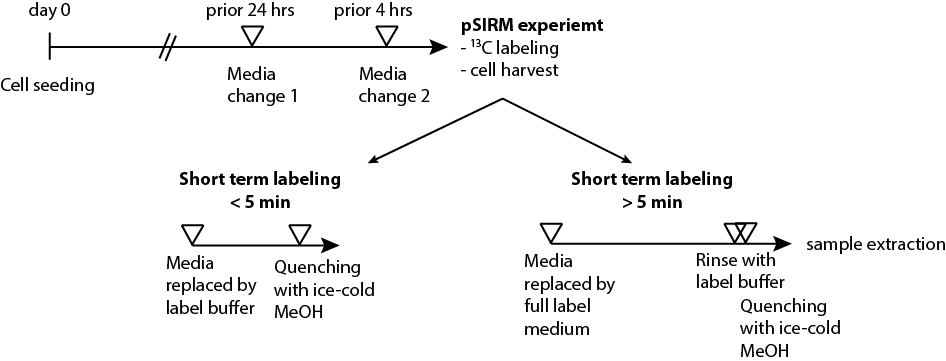
\includegraphics{images/psirm_harvest.png}
\caption{\label{fig:psirmexp}Experimental design of a pSIRM experiment
distuingishing short and long labeling with stable isotopes.}
\end{figure}

For adherent cell cultures only: Include for each experimental condition
an additional petri dish that is solely used to determine the cell count
at the time point of your harvest. This additional plate ensures a
correct determination of absolute quantities and might reduce variation
of pool sizes in the statistical analysis\footnote{Pelleting these cells
  and snap-freezing might give usefull additional samples for western
  blotting.}. Think carefully about control conditions and include cell
culture dishes that are not labeled. These dishes function as a control
for your labeling procedure and the natural abundance of isotopes.

\section{Experimental procedures}\label{experimental-procedures}

There is a slight difference in the protocols for
\protect\hyperlink{psirm:adherent}{adherent} and
\protect\hyperlink{psirm:suspension}{suspension} cells. Please read
instructions and footnotes carefully.

Short\footnote{I would rather recommend this up to 2 min of labeling}
and long term labeling procured differ only in the applied solvents
during the labeling - either label buffer
(\protect\hyperlink{washingbuffer}{LB}) only or a combination of full
label medium (LM) and label buffer (LB). Latter one is applied in order
to remove extracellular metabolites of the media. Both label buffer and
media contain the major nutrients / stable isotopes to keep the main
substrates at constant supply at all times (Table \ref{tab:solvent}).
During the application of stable isotopes longer than a few minutes
cells might sense the absence of further intermediates provided during
standard cell culture procedure and and adjust their metabolic program
accordingly.

\label{tab:solvent}Solvent composition of Full label medium (LM) and label
buffer (BF) for a pSIRM experiment labeling with 13C-glucose.

Solvent

Base

Carbon.source

Supplements

Full label medium (LM)

DMEM, without glucose, glutamine, pyruvate

13C-Glc (2.5 g/L) 12C-Gln (2 mM)

small molecules (inhibitor, antibiotics)

Label buffer (LB)

HEPES (5 mM), NaCl (140 mM), pH 7.4

13C-Glc (2.5 g/L) 12C-Gln (2 mM)

The quality of your data later heavily relies on the exact handling of
the cells and a \emph{consistent timing} throughout the pSIRM
experiment. Especially the step removing the LB and quenching the cells
should be a matter of a tenth of seconds rather than seconds. It is of
great value to perform the cell harvest with a second person.

\section{Protocol pSIRM}\label{protocol-psirm}

\hypertarget{psirm:adherent}{\subsection{Adherent cell
cultures}\label{psirm:adherent}}

The herein described protocols are detailed explanations how to perform
a pSIRM cell harvest for long term label application. If you want to
label for less than 2 minutes omit solely \emph{omit steps 6-8}.

Materials:

\begin{itemize}
\tightlist
\item
  Cell culture dishes, max. confluency 80 \%
\item
  Labeling media (LM) supplemented with substrates (5 ml /
  dish)\footnote{Not required for short term labeling}
\item
  Label buffer (LB) supplemented with substrates (5 ml / dish)
\item
  Ice-cold 50 \% MeOH supplemented with 2 ug/ul cinnamic acid
\item
  2x 5 ml pipette and tips\footnote{Highly recommended, makes labeling
    and harvest super quick}
\item
  Beaker
\item
  Ice
\item
  15 ml falcons (chloroform resistant)
\item
  Cell lifter
\item
  Biological waste bin next to your bench
\end{itemize}

Procedure:

\begin{enumerate}
\def\labelenumi{\arabic{enumi}.}
\tightlist
\item
  Pre-warm LB and LM in the water bath
\item
  Take a number of petri dishes (condition-wise including all biol.
  replicates)
\item
  Discard cell culture media
\item
  Carefully add \emph{long term labeling} LM OR \emph{short term
  labeling}: LB
\item
  Incubate cells on the bench or in an incubator
\item
  Discard LM (beaker)
\item
  Add immediatly 5 ml of LB
\item
  Rotate dish once in order to cover complete surface
\item
  Meanwhile 2nd person get prepared with 5 ml ice-cold MeOH
\item
  Discard LB into beaker and \emph{immediatly} 2nd person quenches with
  ice-cold MeOH
\item
  Collect cell extracts using cell lifter
\item
  Transfer cell extracts into 15 ml falcons
\item
  Store falcons on ice until further processing
\end{enumerate}

Repeat this procedure (step 6-10) for all dishes of a single condition
first. Once MeOH is added metabolic processes are interrupted and cell
extracts can be collected with the help of cell lifter without rush and
subsequently transfered to 15 ml falcon and stored on ice until further
processing (see chapter \protect\hyperlink{ccextraction_meoh}{Cell
extraction methanolic extracts}).

Determine the cell count using your additional petri dishes for each
condition.

\hypertarget{psirm:suspension}{\subsection{Supension cell
cultures}\label{psirm:suspension}}

Materials:

\begin{itemize}
\tightlist
\item
  Cell culture flasks
\item
  Labeling media (LM) supplemented with substrates
\item
  5 ml pipette and tips\footnote{Highly recommended, makes labeling and
    harvest super quick}
\item
  1 ml pipette
\item
  Beaker
\item
  paper tissues
\item
  Liquid nitrogen
\item
  15 ml falcons
\item
  1.5 ml eppendorf tubes
\item
  Biological waste bin next to your bench
\end{itemize}

Procedure:

\begin{enumerate}
\def\labelenumi{\arabic{enumi}.}
\tightlist
\item
  Pre-warm LM in the water bath
\item
  Determine the cell count of your cell suspension(s)
\item
  Take aliquots of \(10-15e+6\) cells and transfer into 15 ml falcon
\item
  Spin down cells very gently 300 g, 2 min at room temperature
\item
  Discard media into beaker
\item
  Resuspend cells gently in three-times 1 ml\footnote{To generate three
    replicates}
\item
  Incubate and keep warm
\item
  Fractionate cell supension in three eppendorf tubes (3x 1 ml each)
\item
  Spin down quickly in top-bench centrifuge\footnote{Most of the times
    30 s are already enough}
\item
  Discard media blandtly on paper tissues
\item
  Snap-freeze immediatly in liquid nitrogen
\item
  Store cells until further processing (see chapter
  \protect\hyperlink{ccextraction_susp}{Cell extraction suspension
  cells})
\end{enumerate}

The important step here to be quick is the alquotation of the cell
suspension and subsequent spin down in the table centrifuge. Suspension
cells are rather small, nevertheless \(3e+6\) cells per extract are a
good starting point for GC-MS measurements.

\section{Hints \& notes}\label{hints-notes}

\begin{itemize}
\tightlist
\item
  The only way to be reproducible and fast is to team up with a second
  person.
\item
  Keep timing consistently through the experiment.
\item
  Keep substrate concentrations constant throughout the experiment in
  all solutions.
\item
  Supplement one stable isotopic labeled substrate with all remaining
  substrates in non-labeled form.
\item
  Think about nutrient levels in your cell culture and your experimental
  conditions. Maybe you want to change things to physiological levels.
\item
  Add additional plate to each condition in order to have material for
  western blotting and others.
\item
  Check carefully the confluency of your dishes and determine seeding
  densities for different conditions.
\item
  In case of small molecule inhibitors: Try to avoid to solve them in
  DMSO - strong impact on chromatography.
\end{itemize}

\chapter{Experimental Protocols}\label{protocols}

\section{Metabolomics sample extraction}\label{extraction}

\subsection{Cell culture experiments}\label{cell-culture-experiments}

\hypertarget{ccextraction_meoh}{\subsubsection{Cell extracts in
MeOH}\label{ccextraction_meoh}}

Materials:

\begin{itemize}
\tightlist
\item
  Chloroform
\item
  15 ml falcon tubes
\item
  thermo or rotary shaker
\end{itemize}

Procedure:

\begin{itemize}
\tightlist
\item
  Add 1 ml chloroform to 5 ml methanolic cell extract
\item
  Incube for 60 min at 4°C on rotary or thermo shaker
\item
  Centrifuge at max speed for 10 min at 4°C
\item
  Collect polar and lipid phases into fresh falcons / tubes
\item
  Dry under vacuum
\end{itemize}

In order to generate technical backups:

\begin{itemize}
\tightlist
\item
  Resuspend dried extracts in 600 ul 20\% MeOH
\item
  Shake at 4°C on thermo shaker for 30 min
\item
  Split volumes into equal parts in fresh eppendorf tubes
\item
  Dry under vacuum
\end{itemize}

Suggested cell density: \(2-3e+6\) cells / extract.

\hypertarget{ccextraction_susp}{\subsubsection{Cell
pellets}\label{ccextraction_susp}}

Materials:

\begin{itemize}
\tightlist
\item
  \protect\hyperlink{mcw}{MCW suppl. cinnamic acid}
\item
  15 ml falcon tubes
\item
  thermo or rotary shaker
\end{itemize}

Procedure:

\begin{itemize}
\tightlist
\item
  Resuspend cell pellets in 1 ml MCW
\item
  Incube for 60 min at 4°C on rotary or thermo shaker
\item
  Add 0.5 ml of H2O to induce phase separation
\item
  Centrifuge at max speed for 10 min, cold temperatures
\item
  Collect polar and lipid phases into fresh falcons / tubes
\item
  Dry under vacuum
\end{itemize}

In order to generate technical backups:

\begin{itemize}
\tightlist
\item
  Resuspend dried extracts in 600 ul 20\% MeOH
\item
  Shake at cold temperature on thermo shaker for 30 min
\item
  Split volumes into equal parts in fresh eppendorf tubes
\item
  Dry under vacuum
\end{itemize}

Suggested cell density: \(2-3e+6\) cells / extract.

\subsection{Tissue samples}\label{tissue-samples}

Materials:

\begin{itemize}
\tightlist
\item
  \protect\hyperlink{mcw}{MCW suppl. cinnamic acid}
\item
  ddH20
\item
  Eppendorf tubes
\item
  Tissue lyzer / pulverizer
\end{itemize}

Procedure:

\begin{itemize}
\tightlist
\item
  Snap-freeze tissue samples
\item
  Pulverize samples
\item
  Aliquote 50 mg of tissue powder
\item
  Add 1.5 ml of MCW (suppl. with cinnamic acid final conc. 2 ug/ul)
\item
  Shake for 60 min on rotary shaker at 4°C
\item
  Add 0.5 ml ddH20 for phase separation
\item
  Centrifuge maximum speed, 10 min at 4°C
\item
  Collect polar and lipid phases in fresh vessels
\item
  Dry under vacuum
\end{itemize}

\subsection{Blood samples}\label{blood-samples}

Material:

\begin{itemize}
\tightlist
\item
  Minivette for capillary blood samples
\item
  \protect\hyperlink{mcw}{MCW suppl. cinnamic acid}
\item
  ddH20
\item
  Eppendorf tubes
\end{itemize}

Procedure:

\begin{itemize}
\tightlist
\item
  Give 20 ul blood / sera directly into 1 ml MCW to avoid lumps
\item
  In case of lumps sonicate samples
\item
  Shake samples at 4°C for 800 rpm for 60 min
\item
  Add 500 ul ddH20 and vortex shortly
\item
  Spin down at 4°C at max speed for 10 min
\item
  Aliquote polar phase into 2-3 times 500 ul in 1.5 ml tubes
\item
  Aliquote lipid phase 2 times in 100 ul lower in 1.5 ml eppi
\item
  Dry in SpeedVac (35°C)
\end{itemize}

\section{Sample derivatisation}\label{sample-derivatisation}

\subsection{Standard protocol}\label{standard-protocol}

Materials:

\begin{itemize}
\tightlist
\item
  Methoxamine (MeOx)
\item
  Pyridine (open under the hood only!)
\item
  MSTFA
\item
  \protect\hyperlink{alkanemix}{Alkane mix} (c10-c36) in Hexane
\item
  Chromacol vials and caps (big, small)
\end{itemize}

Mixtures:

\begin{itemize}
\tightlist
\item
  Solvent 1: 40 mg MeOx in 1 ml Pyridine
\item
  Solvent 2: 10 ul Alkane mix in 1 ml MSTFA
\end{itemize}

Volumens of both solvents are shown for standard (small volumes)
procedures.

Procedure:

\begin{itemize}
\tightlist
\item
  Make sure samples are completly dry (1 h speed vac)
\item
  Add 20 ul (10 ul) of solvent 1 / sample
\item
  Incubate on rotary shaker, 30°C, for 60 min
\item
  Add 80 ul (25 ul) of solvent 2 / sample
\item
  Incubaate on rotary shaker, 37°C, for 90 min
\item
  Centrifuge to spin down insoluble materials
\item
  Prepare aliquotes three times 28 ul or two times 15 ul (small glass
  vials)
\item
  Keep on room temperature until measurement (max. 10 days)
\end{itemize}

\subsection{Specific protocols}\label{specific-protocols}

\subsubsection{Andrash}\label{andrash}

\subsubsection{Fabian}\label{fabian}

\subsubsection{Henning}\label{henning}

\chapter{Data processing - MAUI}\label{proc:maui}

\section{Processing In ChromaToF}\label{processing-in-chromatof}

Create a new folder in ChromaToF Pegasus Acquired Samples and import
your files. The processing of files for Maui-assisted annotation is a
two step process. Therefore two data processing methods have to be set
up and applied to all files.

\subsection{Resampling}\label{resampling}

Resampling is commonly applied and results into a data transformation
enabling an improved detection of low abundant peaks and a reduction of
noise. (Maybe include an example?)

The processing methods requires to tick \texttt{Export\ of\ ...}.
Subsequently, you are asked to define an output folder and the following
paramter:

\begin{itemize}
\tightlist
\item
  Reduction rate: 4
\item
  Beginning to end of the file
\item
  \texttt{.peg}-files
\end{itemize}

\subsection{\texorpdfstring{Combo-export (\texttt{.cdf} \&
\texttt{.csv})}{Combo-export (.cdf \& .csv)}}\label{combo-export-.cdf-.csv}

Re-import the generated \texttt{.peg}-files into a subfolder and apply
the following data processing method.

Activate the box \texttt{asddasd} and define for both file types the
following parameter.

\texttt{.cdf}-file:

\begin{itemize}
\item
  export directory
\item
\end{itemize}

\texttt{.csv}-file:

\begin{itemize}
\item
  export directory
\item
\end{itemize}

\section{Maui notes}\label{maui-notes}

\section{Maui exports}\label{mauiexport}

With initiation of a project folder via \texttt{MTXQCvX2\_init.Rmd} you
created an \texttt{input}-folder containing three subfolders:
\texttt{gc}, \texttt{inc}, \texttt{quant}. In the following all files
that should be exported and copied into these folders are described in
detail.

\subsection{\texorpdfstring{\texttt{input/gc/...}}{input/gc/...}}\label{inputgc...}

Four input files are exported in order to assess the quality of the
GC-MS performance of the run. The menue \texttt{Diagnostics} is
selectable via right click on your Maui project name. Only the cinnamic
acid peak areas are exported via the function
\texttt{Export\ Quantification} with right click on the actual
container.

Exported Files:

\begin{itemize}
\tightlist
\item
  \texttt{Alcane\_intensities.csv} - Diagnostics/Export Alcane
  intensities
\item
  \texttt{InternalStandard.csv} - cinAcid container, Export
  quantification, rename!
\item
  \texttt{MassSum-73.csv} - Diagnostics/QC Mass Sum Export; enter: 73
  for m/z 73
\item
  \texttt{PeakDensities-Chroma.csv} - Diagnostics/ExportPeakDensities
\end{itemize}

\subsection{\texorpdfstring{\texttt{input/quant/...}}{input/quant/...}}\label{inputquant...}

Only one container has to be exported and contains the peak areas of
each metabolite and measurement. Keep in mind that you should have
uploaded \texttt{pTop5\ mass\ list} for the correct determination of
peak areas in case of labeling with stable isotopes.

A further note - Maui performs absolute quantification and stores values
in the \texttt{samplePeakGroups-QMQ} container. These quantities are
determined by polynominal regression, and not linear regression.

The file \texttt{ManualQuantTable.tsv} is automatically generated by
Maui during processing the absolute quantification.

Exported Files:

\begin{itemize}
\tightlist
\item
  \texttt{ManualQuantTable.tsv} - location:
  \texttt{Maui-project/export/QM-AbsoluteQuantification/...}\footnote{Don´t
    forget to rename it - e.g., e17123cz}
\item
  \texttt{quantMassAreasMatrix.csv} - Quantification export of the
  container \texttt{samplesPeakGroups}
\end{itemize}

\subsection{\texorpdfstring{\texttt{input/inc/...}}{input/inc/...}}\label{inputinc...}

This exports are only required in case of an experiment including the
application of stable isotopes. It´s this the case you should have
performed two things:

\begin{enumerate}
\def\labelenumi{\arabic{enumi}.}
\tightlist
\item
  Used the optional upload of \texttt{pTop5\ mass\ list}
\item
  Go through the pSIRM workflow in Maui
\end{enumerate}

Exported Files:

\begin{itemize}
\tightlist
\item
  \texttt{DataMatrix.csv} - Export \% Label of container
  \texttt{pSIRM-samplesPeakGroups}
\item
  \texttt{pSIRM\_SpectraData.csv} - pSIRM Spectra Export of container
  \texttt{pSIRM-samplesPeakGroups}\footnote{Requires the selection of
    Natural\_MIDs.txt}
\end{itemize}

\chapter{Data Processing - Metmax}\label{proc:metmax}

\section{Resampling}\label{resampling-1}

\section{1D-basic}\label{d-basic}

\section{Reference search}\label{reference-search}

\section{Export for Metmax}\label{export-for-metmax}

\section{Data extraction with Metmax}\label{data-extraction-with-metmax}

\subsection{Peak areas}\label{peak-areas}

\subsection{MIDs}\label{mids}

\chapter{Solutions and Materials}\label{mm}

\section{Solutions}\label{solutions}

\hypertarget{washingbuffer}{\subsection{Label
buffer}\label{washingbuffer}}

Materials:

\begin{itemize}
\tightlist
\item
  ddH2O (500 ml)
\item
  140 mM NaCl (4.1 g)
\item
  5 mM Hepes (0.569 g)
\item
  pH calibration 7.4
\end{itemize}

Procedure:

\begin{itemize}
\tightlist
\item
  Weigh the correct amounts of Hepes and NaCl
\item
  Resolve in a glas bottle with 450 ml of water
\item
  Stir carefully
\item
  Check and adjust pH
\item
  Adjust volumes to 500 ml
\end{itemize}

\hypertarget{mcw}{\subsection{MCW}\label{mcw}}

Materials:

\begin{itemize}
\tightlist
\item
  Methanol
\item
  Chloroform
\item
  ddH2O
\item
  Cinnamic acid stock in MeOH (2 mg/ml): final conc. 2 ug/ml
\end{itemize}

Procedure:

\begin{itemize}
\tightlist
\item
  Mix the solvents in the ratio of volumes - Methanol:Chlorofom:Water --
  5:2:1
\item
  Supplement cinnamic acid stock 1:1000
\item
  Store at -25°C
\end{itemize}

\hypertarget{alkanemix}{\subsection{Alkane-Mix}\label{alkanemix}}

Materials:

\begin{itemize}
\tightlist
\item
  Hexane
\item
  Alkanes: c10, c12, c15, c17, c19, c22, c28, c32, c36
\item
  Thermo mixer
\item
  Glass vials and caps
\end{itemize}

Procedure:

\begin{itemize}
\tightlist
\item
  Prepare stock solutions in hexane:
\item
  c10 - c17 (liquid): 25 ul/ml
\item
  c19 - c32: 20 mg/ml
\item
  c36: two-times 15 mg/1.5 ml
\item
  Warm up alkane stocks in thermo mixer 40°C
\item
  Prepare a text mixture in equal amounts, e.g., 50 ul each, but use
  twice the volume of c36
\item
  Mix test mixture with MSTFA: 10 ul / 1 ml MSTFA
\item
  Check alkane profile by GC-MS
\item
  If required: adjust volumes and re-test or create larger volume of
  zour mixture for aliquots
\item
  Store aiquots in glass vials, close well and store at 4°C
\item
  For usage: gently warm up glass vials at 30 C on thermo mixer for 10
  min and vortex before adding it to the MSTFA
\end{itemize}

Adjust the volumes of the alkane stocks in order to create a curve
shaped distribution of all alkanes in the chromatogram: lower
intensities for c10 and c32-36, slowly increasing intensities for the
alkanes in between.

\section{Materials}\label{materials}

\label{tab:chemicals}List of chemicals including company names and catalog
number.

Chemical

Catalog.Nb

Company

Storage

Chloroform

132950-1L

Sigma

RT

Cinnamic acid

C80857 5g

Aldrich

RT

Hexane for HPLC \textgreater{} 97\% (GC)

34859-1L

Sigma

RT

Methanol

1060351000

Merck

RT

Methoxyamine hydrochloride

226904-5G

Aldrich

RT

MSTFA - Methyltrimethylsilyltrifluoracetamide

701270201

Macherey-Nagel

4°C

Pyridine

270970-100ML

Sigma

RT

\chapter{Output tables}\label{output}

\section{Project-files}\label{o_project}

\subsection{\texorpdfstring{\texttt{MTXQC\_params.csv}}{MTXQC\_params.csv}}\label{mtxqc_params.csv}

Parameter

Description

Value

inputformat

Format of input files

maui

ann

File name of the annotation file

annotation.csv

sample\_ext

File name of the file containing cell counts or extracted tissue weight,
volumes of blood

Sample\_extracts.csv

instd

Internal extraction standard present

TRUE

addQ

Additional quantification standards measured?

no

addQ\_Int

Integration of additional quantification standards in all batches of the
MTXQC project

no

substr

Applied stable isotopes

glc

quant\_vol

Dried volume of polar phase of quantification standards in uL

500

backups

Preparation of technical aliquots

2

samples

Origin of samples

cell extracts

subf

subfolder or project folder

psirm\_glucose/

data

Nature of the experiment

pSIRM

quant

Version of quantification standards

Quant1\_v4

\subsection{\texorpdfstring{\texttt{Maui\_params.csv}}{Maui\_params.csv}}\label{maui_params.csv}

Parameter

Description

Value

spath

subfolder or project folder

psirm\_glucose/

matrix

Input file containing all peak areas

quantMassAreasMatrix.csv

mz

Input file containing m/z intensities

MassSum-73.csv

mid

Input file containing MIDs for each intermediate and file

pSIRM\_SpectraData.csv

inc\_data

Input file containing calculated stable isotope incorporation in the
format 100 percent = 1

DataMatrix.csv

inputformat

Input format type

maui

intstd

If MTXQC project contains an internal extraction standard

TRUE

alkanes

If MTXQC project contains evaluation of alkane profile

TRUE

peakchroma

If MTXQC project contains evaluation of derivatisation efficiency

TRUE

mqt

If MTXQC project includes absolute quantification

TRUE

inc

If MTXQC project includes labeling with stable isotopes

TRUE

\subsection{\texorpdfstring{\texttt{Metmax\_params.csv}}{Metmax\_params.csv}}\label{metmax_params.csv}

\section{\texorpdfstring{\texttt{output/gc/...}}{output/gc/...}}\label{outputgc...}

\subsection{\texorpdfstring{\texttt{HM\_GC\_values.csv} \&
\texttt{qcmetric\_xy.csv}}{HM\_GC\_values.csv \& qcmetric\_xy.csv}}\label{hm_gc_values.csv-qcmetric_xy.csv}

MTXQC exports a file summarising quality factors for each of the four
parameter evaluating the GC performance. A summary representing the
values illustrated in the heatmap are shown in table
\href{@ref(tab:o_hm_gc)}{\texttt{HM\_GC\_values.csv}}, individual
exports for each metric in table
\href{@ref(tab:o_gc_metric)}{\texttt{qcmetric\_xy.csv}}.

Column.name

Description

Value

Batch\_Id

Batch-Id

e18274ba

qc\_metric

QC metric factor corresponding with 1 - very good and 0 - very low

0.937254457

title

Class of QC metric

alkanes

Column.name

Description

Value

Batch\_Id

Batch-Id

e18274ba

qc\_metric

QC metric factor corresponding with 1 - very good and 0 - very low

0.937254457

title

Class of QC metric

alkanes

\subsection{\texorpdfstring{\texttt{IntStandard\_normfactors.csv} \&
\texttt{IntStandard\_stats.csv}}{IntStandard\_normfactors.csv \& IntStandard\_stats.csv}}\label{intstandard_normfactors.csv-intstandard_stats.csv}

Column.name

Description

Value

File

File name

e18274ba\_17.cdf

PeakArea

Peak area of internal extraction standard

89308492

Batch\_Id

Bacth-Id

e18274ba

IntStd\_fac

Determined normalisation factor

0.837457514

IntStd\_eval

Evaluation of normalisation factor in relation to defined range
plus/minus one standard deviation

within

Column.name

Description

Value

File

File name

e18274ba\_17.cdf

PeakArea

Peak area of internal extraction standard

89308492

Batch\_Id

Batch-Id

e18274ba

IntStd\_fac

Normalisation factor

0.837457514

IntStd\_eval

Evaluation regarding QC

within

n\_batch

Number of annotated intermediates

54

mean\_batch

Mean value of internal standard peak area across the batch

106642415.3

sd\_batch

Standard deviation of the peak area across the batch of the internal
extraction standard

36710894.86

\subsection{\texorpdfstring{\texttt{Min\_Annotation.csv} \&
\texttt{SumArea\_stats.csv}}{Min\_Annotation.csv \& SumArea\_stats.csv}}\label{min_annotation.csv-sumarea_stats.csv}

Column.name

Description

Value

File

File name

e18274ba\_17.cdf

Batch\_Id

Extracted Batch-Id derived from file name

e18274ba

n\_area

Number of peak areas per file

101

sum\_area

Sum of all peak areas

44614610885

n\_total

Total number of entries (including NA)

107

mean\_batch

Mean value of peak areas across the batch

34409759414

sd\_batch

Standard deviation of peak areas across the batch

12913422445

area\_fac

Normalisation factor of the file

1.296568521

n\_50

Number of annotated peak areas per file corresponding to fifty percent
of maximum number of annotated peaks in the batch

53.5

Column.name

Description

Value

Batch\_Id

Batch-Id

e18274ba

n\_50

Number corresponding to fifty percent of the maximum number of annotated
peaks per file

53.5

\subsection{\texorpdfstring{\texttt{mz73\_data.csv}}{mz73\_data.csv}}\label{mz73_data.csv}

Column.name

Description

Value

File

File name

e18274ba\_17.cdf

Batch\_Id

Batch-ID

e18274ba

mean\_73

Mean value of the sum of m/z 73 intensities per file

16314646.1

sd\_73

Standard deviation of the mean of the sum of m/z 73 intensities per file

143890119.5

n\_peaks

Number of intensities used for statistics

600

sum\_area

Sum of all m/z intensities

6777312761

ratio\_total

Ratio of sum\_area in relation to the sum of all annotated peak areas

0.002407244

\section{\texorpdfstring{\texttt{output/quant/...}\{o\_quant\}}{output/quant/...\{o\_quant\}}}\label{outputquant...o_quant}

\subsection{\texorpdfstring{\texttt{calcheck\_linearity.csv}}{calcheck\_linearity.csv}}\label{calcheck_linearity.csv}

Column.name

Description

Value

Metabolite

Full library name of the metabolite

Alanine\_(3TMS)\_MP\_RI:1367\_IDENT:B+C

Batch\_Id

Batch-Id

e18274ba

File

File name

e18274ba\_53.cdf

QuantMasses

Defined quantification masses

110.0 133.0 114.0 100.0 188.0 190.0

PeakArea

Sum of peak areas based on defined QuantMasses

12710956

Type

Kind of sample

sample

Metabolite\_manual

Manual defined metabolite name

\#Alanine (3TMS)

Metabolite\_short

Short version of metabolite name

Alanine\_(3TMS)

Lettercode

Lettercode version of metabolite name

Ala\_3TMS

Q1\_value

Quantity in the quantification standard Q1:1 if included in pmol

x

Mass\_Pos

m/z value that should be evaluated in case of the application of
isotopes

190

SE\_sel

Intermediate used for evaluation of MIDs if present

x

Q\_sel

Intermediate used for absolute quantification if Q1:1 present

x

nopsirm

If exclusivly used for quantification purposes only

Standards

Origin

Quantification standard

Qstd

adj\_r\_squared

Adjusted Rsquare value of linear regression of the calibration curve

0.997002799

slope

Slope of the calibration curve determined by linear regression

0.000578604

intercept

Intercept of the calibration curve determined by linear regression

-898.3400476

calc\_curve

Calibration curve available for absolute quantification

yes\_cal

islinear

Evaluation of peak area in relation to linear range of the calibration
curve

linear

\subsection{\texorpdfstring{\texttt{CalculationFileData.csv}}{CalculationFileData.csv}}\label{calculationfiledata.csv}

Column.name

Class

Description

Value

Batch\_Id

AnnExp

Batch-Id extracted from file name

e18274ba

CL

AnnExp

Experimental parameter

BE(2)-C

Cond

AnnExp

Experimental parameter

Control

File

AnnExp

File name

e18274ba\_25.cdf

Standards

AnnExp

Defined as standard (InternalStandard, Alk)

Time

AnnExp

Experimental parameter

0

Type

AnnExp

Type of measurement

sample

Extract\_vol

AnnExtract

Defined extractes in count, mg or uL defined in Unit

3290000

Unit

AnnExtract

Defined unit for corresponding Extract\_vol

count

Lettercode

AnnMet

Lettercode version of metabolite name

Glyc3P

Metabolite

AnnMet

Library name

Glycerol-3-phosphate\_(4TMS)\_MP\_RI:1756\_IDENT:B+C

Metabolite\_manual

AnnMet

Manual defined metabolite name

\#Glycerol-3-phosphate (4TMS)

Metabolite\_short

AnnMet

Short version of library name

Glycerol-3-phosphate\_(4TMS)

absconc

CalCurve

Absolute quantity in pmol

24061.77157

adj\_r\_squared

CalCurve

Adjusted Rsquare value of calibration curve

0.999667641

calc\_curve

CalCurve

Relation of peak area to calibration curve

yes\_cal

intercept

CalCurve

Intercept of calibration curve

234.0083706

islinear

CalCurve

Classification of peak area

linear

Origin

CalCurve

Source of Quant1:1 value

Qstd

Q1\_value

CalCurve

Quantity defined in Q1:1 standard

x

slope

CalCurve

Slope of calibration curve

0.000821689

corr\_absconc

ExtrFactor

Corrected absolute quantities by extraction factor

16041.18105

extr\_fac

ExtrFactor

Extraction factor derived from MTXQC\_params

0.666666667

Mass\_Pos

MTXQCsettings

m/z-value (m\_inc) used for determination of stable isotope
incorporation

359

nopsirm

MTXQCsettings

Exclusivly used for absolute quantification

Q\_sel

MTXQCsettings

Used for absolute quantification

x

QuantMasses

MTXQCsettings

Defined quantification masses

101.0 299.0 133.0 357.0 103.0 359.0

SE\_sel

MTXQCsettings

Evaluation of MIDs if available

x

IntStd\_eval

Norm\_InternalStd

Evaluation of internal extraction standard

within

IntStd\_fac

Norm\_InternalStd

Normalisation factor based on internal extraction standard

1.090830836

area\_fac

Norm\_SumOfArea

Normalisation factor for sum of area normalisation

0.507591279

sum\_area

Norm\_SumOfArea

Sum of all peak areas of the file

17466093782

Conc\_microM

Quantities

Quantities in (micromolar) only determined for extracted volumes

NA

Conc\_pmio

Quantities

Quantities in (pmol)

4875.73892

IntStd\_Conc

Quantities

Quantities in (pmol) after normalisation with internal standard factor

14705.47084

IntStd\_Conc\_microM

Quantities

Quantities in (micromolar) after normalisation with internal standard
factor: only for volumes

NA

IntStd\_Conc\_pmio

Quantities

Quantities in (pmol/unit) after normalisation with internal standard
factor

4469.747976

IntStd\_sumA\_Conc

Quantities

Quantities in (pmol) after normalisation with internal standard factor
and sum of area normalisation

28971.0865

IntStd\_sumA\_Conc\_pmio

Quantities

Quantities in (pmol/per unit) after normalisation with internal standard
factor and sum of area normalisation

8805.801367

PeakArea

Quantities

Determined peak area based on QuantMasses

28998527

sumA\_Conc

Quantities

Quantities in (pmol) after sum of area normalisation

31602.5545

sumA\_Conc\_microM

Quantities

Quantities in (micromolar) after sum of area normalisation

NA

sumA\_Conc\_pmio

Quantities

Quantities in (pmol/per unit) after sum of area normalisation

9605.639664

\subsection{\texorpdfstring{\texttt{HeatMap\_Quant\_pTop5.csv}}{HeatMap\_Quant\_pTop5.csv}}\label{heatmap_quant_ptop5.csv}

Column.name

Description

Value

Lettercode

Short name of metabolite

Cit

Batch\_Id

Batch-Id

e18274ba

Metabolite

Library name of metabolite

Citric acid\_(4TMS)\_MP\_RI:1814\_IDENT:B+D

Par

Parameter

R2\_cal

Val

Value of the parameter for corresponding metabolite

0.996053496

\subsection{\texorpdfstring{\texttt{pTop5\_Calibration\_Samples\_lincheck.csv}}{pTop5\_Calibration\_Samples\_lincheck.csv}}\label{ptop5_calibration_samples_lincheck.csv}

Column.name

Description

Value

Lettercode

Short name of metabolite

3PGA

islinear

Evaluation of peak area in relation to calibration curve if available

NaCal

Batch\_Id

Batch-Id

e18274ba

Origin

Origin of Quant1:1-value

NA

count

Number of peak areas

51

sum\_lin

Sum of peak area per islinear level

51

prop

Fraction of count to sum\_lin

1

\subsection{\texorpdfstring{\texttt{top5\_CalibrationInfo\_unique.csv}}{top5\_CalibrationInfo\_unique.csv}}\label{top5_calibrationinfo_unique.csv}

Column.name

Description

Value

Metabolite

Library name of metabolite

Citric acid\_(4TMS)\_MP\_RI:1814\_IDENT:B+D

Lettercode

Lettercode name of metabolite

Cit

Batch\_Id

Batch-Id

e18274ba

Origin

Origin of quant1:1 value

Qstd

adj\_r\_squared

Adjsuted Rsquare of calibration curve

0.996053496

intercept

Intercept of calibration curve

564.549288

slope

Slope of calibration curve

0.000194064

Frac\_calcurve

Fraction of peak area in linear range of calibration curve

10

\subsection{\texorpdfstring{\texttt{top5\_QMQcurveInfo.csv}}{top5\_QMQcurveInfo.csv}}\label{top5_qmqcurveinfo.csv}

Column.name

Description

Value

Lettercode

Lettercode of metabolite name

Cit

Letter\_Derivate

Derivate name

Cit

Quant1\_v4

Quant1:1 value in (pmol)

52050

Metabolite

Library name of metabolite

Citric acid\_(4TMS)\_MP\_RI:1814\_IDENT:B+D

Batch\_Id

Batch-Id

e18274ba

Dilution

Dilution factor

0.2

ChromIntensities

Corresponding peak areas

45074572

Concentration

Concentration in (pmol)

10410

Origin

Origin of quantification standard

Qstd

Metabolite\_short

Short name of metabolite

Citric acid 275\_(4TMS)

adj\_r\_squared

Adjusted Rsquare of calibration curve

0.996053496

intercept

Intercept of calibration curve

564.549288

slope

Slope of calibration curve

0.000194064

max

Max. value of calibration curve

52050

min

Min. value of calibration curve

260.25

\section{\texorpdfstring{\texttt{output/inc/...}}{output/inc/...}}\label{outputinc...}

\subsection{\texorpdfstring{\texttt{HeatMap\_Incorporation.csv}}{HeatMap\_Incorporation.csv}}\label{heatmap_incorporation.csv}

Column.name

Description

Value

Lettercode

Lettercode name of metabolite

3PGA

Batch\_Id

Batch-Id

e18274ba

Par

Parameter

NA\_count

Val

Value of the parameter shown in heatmap

0.740740741

\subsection{\texorpdfstring{\texttt{SE\_calculation\_NAscore.csv}}{SE\_calculation\_NAscore.csv}}\label{se_calculation_nascore.csv}

Column.name

Description

Value

Lettercode

Lettercode name of metabolite

Cit

Batch\_Id

Batch-Id

e18274ba

na\_frac\_r

Class of NA-value

0

N

Number of MIDs

46

fracr\_prop

Fraction of MIDs with x NA-values in relation to total number of
evaluated MIDs

0.851851852

\subsection{\texorpdfstring{\texttt{SE\_classification.csv}}{SE\_classification.csv}}\label{se_classification.csv}

Column.name

Description

Value

Lettercode

Lettercode name of metabolite

Cit

Batch\_Id

Batch-Id

e18274ba

File

File name

e18274ba\_26.cdf

sum\_spa

\emph{expl}

4297

sum\_bpa

\emph{expl}

1861

low3a\_ratio

\emph{expl}

2.30897367

rel\_sb

\emph{expl}

higher

val\_score

Validation score

confident

count\_score

MID evaluation

goodQ

\subsection{\texorpdfstring{\texttt{SE\_validation.csv}}{SE\_validation.csv}}\label{se_validation.csv}

Column.name

Description

Value

Lettercode

Lettercode name of metabolite

Cit

Batch\_Id

Batch-Id

e18274ba

count\_score

Evaluation of MID

goodQ

N\_count

Number of evaluated MIDs

54

sum\_files

Number of detected MIDs

54

prop

Proportion of MIDs for count\_score level

1

\chapter{Frequently Asked Questions}\label{FAQ}

\section{What are additional quantification
standards}\label{what-are-additional-quantification-standards}

\section{How do I extend
conversion\_metabolite.csv}\label{how-do-i-extend-conversion_metabolite.csv}

\chapter{GC-MS settings}\label{gcms}

In the following paragraphs details of GC-MS settings are described in
detail. The herein described settings have been optimized for cell
extracts measured in split-mode 1:5 on the instrument Pegasus 4D-C
GC-ToF-MS in 1D mode equiped with an autosampler Gerstel MPS.

\subsection{Autosampler settings}\label{autosampler-settings}

The table \ref{tab:gerstel} summarises the defined parameter for method
settings of the Gerstel MPS.

\label{tab:gerstel}Parameter of Gerstel MPS settings

Part

Parameter

Value

System

Runtime

40 min

System

GC Cool down time

3 min

System

Cryo Timeout

15 min

MPS - Liquid Injection

Syringe

10ulALX

MPS - Liquid Injection

Sandwhich

No Sandwhich

MPS - Liquid Injection

Inj. Volume (uL)

0.8

MPS - Liquid Injection

Air Volume below (uL)

1

MPS - Liquid Injection

Inj. Speed (uL/s)

20

MPS - Liquid Injection

Fill Volume (uL)

4

MPS - Liquid Injection

Fill Strokes for Sample

6

MPS - Liquid Injection

Fill Speed (uL/s)

1

MPS - Liquid Injection

Eject Speed (uL/s)

20

MPS - Liquid Injection

Viscosity Delay (s)

1

MPS - Liquid Injection

Pre Inj. Delay (s)

0

MPS - Liquid Injection

Post Inj. Delay (s)

0

MPS - Liquid Injection

Inj. Penetration (mm)

30

MPS - Liquid Injection

Sample Tray Type

VT98

MPS - Liquid Injection

Vial Penetration (mm)

32

MPS - Rinse

Wash1 Preclean

2

MPS - Rinse

Wash1 Postclean

3

MPS - Rinse

Wash1 Preclean

2

MPS - Rinse

Wash1 Postclean

3

MPS - Rinse

Sample (4.0 uL)

0

MPS - Rinse

Rinse Fill speed (uL/s)

1

MPS - Rinse

Viscosity Delay (s)

1

MPS - Rinse

Eject Speed (uL/s)

20

The injector itself is a temperature-regulated system providing the
advantage of a focused injection of the sample. Gradient

\begin{figure}
\centering
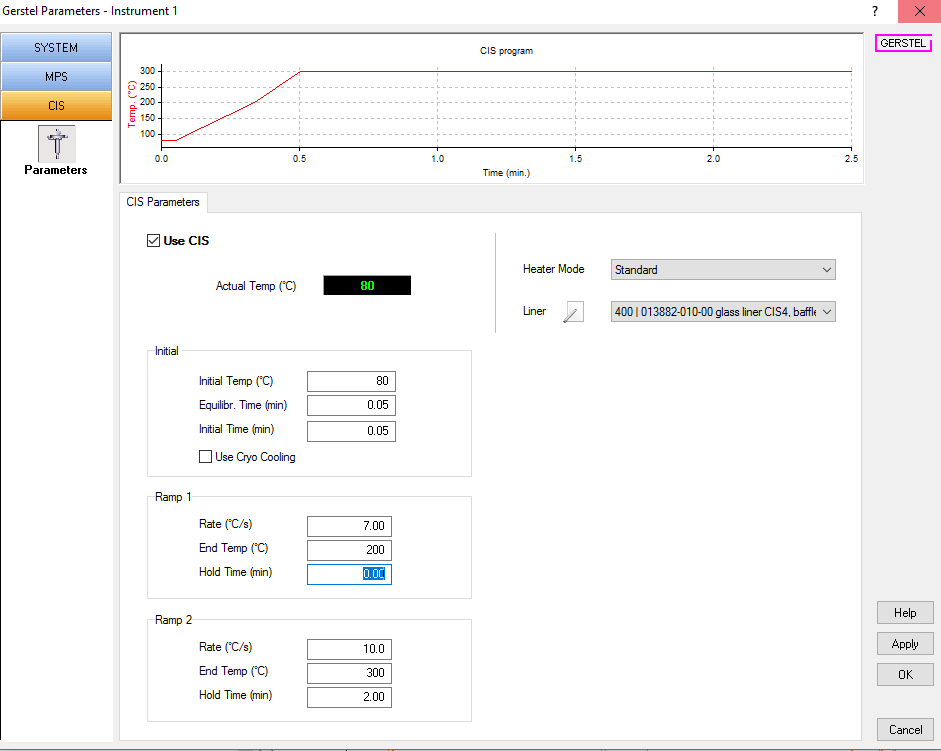
\includegraphics{images/cis.PNG}
\caption{\label{fig:cis}Settings temperature-regulated injection for Gerstel
MPS}
\end{figure}

\subsection{Gas chromatography}\label{gas-chromatography}

The most important settings of the GC method are listed below. A
graphical representation of the gradient in the oven is shown in figure
\ref{fig:gradient} and corresponding values in table
\ref{tab:gradient2}.

Flow path:

\begin{enumerate}
\def\labelenumi{\arabic{enumi}.}
\tightlist
\item
  Inlet: Front
\item
  Capillary: GC Oven 50 m, 250 u int. diameter, 0.25 u film thickness,
  RTX-5 phase
\item
  Capillarty: Detector 0.21 m, 250 u int. diameter, 0.25 u film
  thickness, RTX-5 phase
\item
  Detector: TOF
\end{enumerate}

Additional parameter:

\begin{itemize}
\tightlist
\item
  Carrier Gas: Helium
\item
  Transfer line Temperature (°C): 250
\end{itemize}

Front Inlet:

\begin{itemize}
\tightlist
\item
  Mode: split / splitless
\item
  Flow: 1.2 mL/min, entire run
\item
  Septum Purge Flow: 0 mL/min
\item
  Temperature: Initial - 200°C; duration 0 min
\end{itemize}

Oven:

\begin{itemize}
\tightlist
\item
  Equilibration time (s): 60
\item
  Modulator enabled: yes
\item
  Modulator offset (°C): 5
\end{itemize}

\begin{figure}
\centering
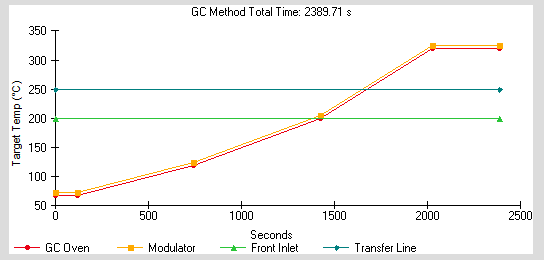
\includegraphics{images/gradient.PNG}
\caption{\label{fig:gradient}GC gradient - graphical representation. Rate in
(°C/min), Target temperature in (°C), Duratin in (min).}
\end{figure}

\label{tab:gradient2}GC gradient profile in numbers.

Rate

Target\_Temp

Duration

Initial

68

2

5

120

0

7

200

0

12

320

6

\subsection{Mass spectrometer
settings}\label{mass-spectrometer-settings}

\bibliography{book.bib,packages.bib}


\end{document}
